\documentclass{article}
\usepackage{tikz, tikz-3dplot}
\begin{document}
    \begin{center}
        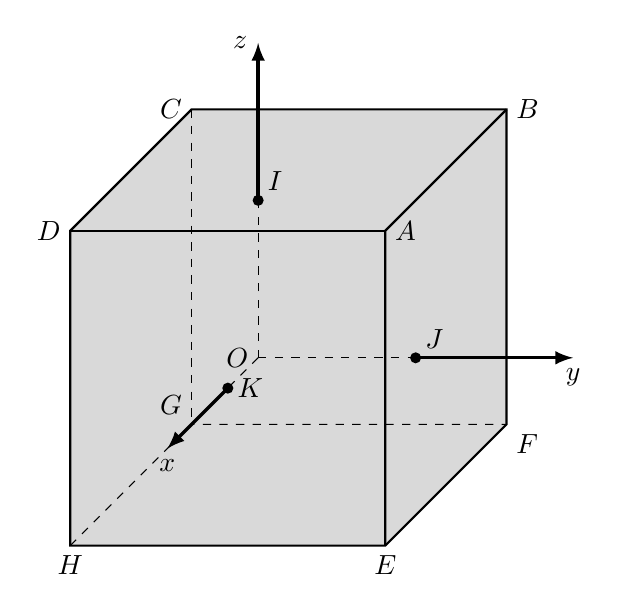
\begin{tikzpicture}
        %x->y, y->z, z->x
        \coordinate (A) at (2,2,1);
        \coordinate (B) at (2,2,-3);
        \coordinate (C) at (-2,2,-3);
        \coordinate (D) at (-2,2,1);
        \coordinate (E) at (2,-2,1);
        \coordinate (F) at (2,-2,-3);
        \coordinate (G) at (-2,-2,-3);
        \coordinate (H) at (-2,-2,1);
        \coordinate (I) at (0,2,0);
        \coordinate (J) at (2,0,0);
        \coordinate (K) at (0,0,1);
        \coordinate (O) at (0,0,0);

        \draw[thick, fill=gray!30] (H) -- (E) -- (F) -- (B) -- (C) -- (D) -- cycle;
        \draw[thick] (E) -- (A) -- (B);
        \draw[thick] (D) -- (A);
        \draw[dashed] (H) -- (G) -- (F);
        \draw[dashed] (C) -- (G);

        \draw[thin, dashed] (O) -- (J);
        \draw[very thick, ->, >=latex] (J) -- (4,0,0) node[below]{\(y\)};

        \draw[thin, dashed] (O) -- (I);
        \draw[very thick, ->, >=latex] (I) -- (0,4,0) node[left]{\(z\)};

        \draw[thin, dashed] (O) -- (K);
        \draw[very thick, ->, >=latex] (K) -- (0,0,3) node[below]{\(x\)};

        \node at (A) [right]{$A$};
        \node at (B) [right]{$B$};
        \node at (C) [left]{$C$};
        \node at (O) [left] {$O$};
        \node at (E) [below]{$E$};
        \node at (F) [below right]{$F$};
        \node at (D) [left]{$D$};
        \node at (G) [above left]{$G$};
        \node at (H) [below]{$H$};
        \node at (I) [above right]{$I$};
        \node at (J) [above right]{$J$};
        \node at (K) [right]{$K$};
        \fill (I) circle(2pt);
        \fill (J) circle(2pt);
        \fill (K) circle(2pt);
        \end{tikzpicture}

    \end{center}
\end{document}